\documentclass[11pt]{article}

% 页面设置
\usepackage[top=1cm, bottom=2cm, left=1cm, right=1cm]{geometry}

% 中文支持
\usepackage{ctex}

% 数学包
\usepackage{amsmath, amssymb, amsthm}

% 算法包
\usepackage[linesnumbered, ruled]{algorithm2e}

% 颜色和命令定义
\usepackage{xcolor, xparse}

% 代码显示
\usepackage{listings}

% 图形包
\usepackage{graphicx}

% 子图包
\usepackage{subcaption}

% 表格包
\usepackage{booktabs}

% 其他需要的包
\usepackage{mathrsfs}
\usepackage{wrapfig}
\usepackage{forest}
\usepackage[normalem]{ulem} % 保持 \emph 为斜体
\usepackage{bm}
\usepackage{multicol}
\usepackage{verbatim}
\usepackage{float}
\usepackage{pifont}
\usepackage{enumitem} % 使用更多的列表标签
\usepackage{caption}


% 添加 'soul' 包用于高亮和支持换行
\usepackage{soul}

% 定义自定义颜色
\definecolor{cmdbg}{RGB}{220, 220, 220} % 浅灰色背景

% 设置高亮颜色
\sethlcolor{cmdbg}

% 定义 \ccmd 命令,用于行内代码片段
\newcommand{\ccmd}[1]{\texttt{\hl{#1}}}

% 超链接(放在最后)
\usepackage[colorlinks=true, linkcolor=blue]{hyperref}

\author{
    \makebox[0.8\textwidth]{%
        \centering
        杨远青 \quad 22300190015 \quad
        \href{https://github.com/bud-primordium/Computational-Physics-Fall-2024}{\raisebox{-2pt}{
\includegraphics[height=12pt]{comphys.pdf}}}
    }
}



\title{基于M\"{u}ller--Brown势的神经网络建模\\}

\begin{document}
\maketitle
% \textit{正面迎击ddl军团!}


\section{问题描述}
\subsection{函数定义}
M\"{u}ller--Brown势能函数解析式为:
\[
    U(x_1, x_2) = s \cdot \sum_{k=1}^4 A_k \exp\left[
        \alpha_k (x_1 - a_k)^2 + \beta_k (x_1 - a_k)(x_2 - b_k) + \gamma_k (x_2 - b_k)^2
        \right]
\]
\subsection{参数系统}
\begin{minipage}[t]{0.5\textwidth}
    \vspace{-\baselineskip}
    \begin{align*}
        \text{振幅系数:}  & \quad \bm{A} = (-200, -100, -170, 15)     \\
        \text{二次项参数:} & \quad
        \begin{aligned}[t]
            \bm{\alpha} & = (-1, -1, -6.5, 0.7)   \\
            \bm{\beta}  & = (0, 0, 11, 0.6)       \\
            \bm{\gamma} & = (-10, -10, -6.5, 0.7)
        \end{aligned}                     \\
        \text{中心坐标:}  & \quad
        \begin{aligned}[t]
            \bm{a} & = (1, 0, -0.5, -1) \\
            \bm{b} & = (0, 0.5, 1.5, 1)
        \end{aligned}                               \\
        \text{缩放因子:}  & \quad s = 0.05                            \\
        \text{定义域:}   & \quad x_1 \in (-1.5,1),\ x_2 \in (-0.5,2) \\
        \text{势能截断:}  & \quad U \leq  U_{\text{cut}} = 9          \\
    \end{align*}
\end{minipage}
\hfill
\begin{minipage}[t]{0.48\textwidth}
    \vspace{-\baselineskip}
    \centering
    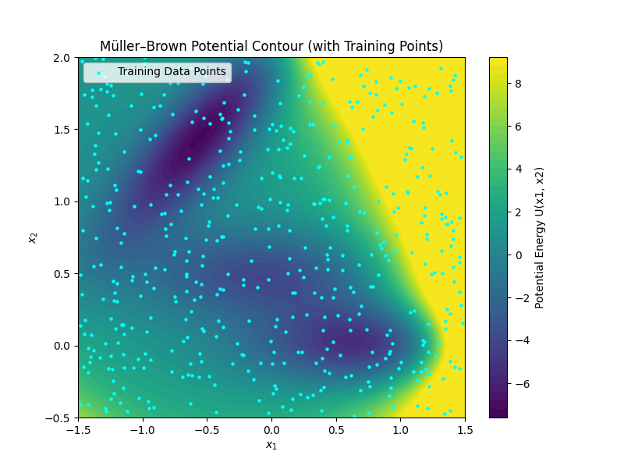
\includegraphics[width=\linewidth]{potential_data.png}
    \captionof{figure}{势能面与训练集可视化}
    \label{fig:surface}
\end{minipage}
\end{document}